\section{Comparison between Controller Designs}\label{sec:comparison}
The two controller designs are now compared in order to analyze the robustness and the performance. The control inputs applied by each controller are also compared. The simulations carried out in this section include input disturbances, both from wind, current and waves, and measurement noise in the outputs. The measurement noise are modeled to have a power spectral density similar to the sensor noise that comes out of the sensor fusion. Parameter variations are also included.

The performance comparison is evaluated by looking at the response of the model of the system when tracking a step in the reference inputs, $\dot{x}_\mathrm{b,ref}$ and $\psi_\mathrm{ref}$. 

The disturbances applied to the system range from $\pm$\num{1.5} N in the force along the $\dot{x}_\mathrm{b}$ axis and $\pm$\num{1.5} Nm in the torque around the $z_\mathrm{b}$ axis. These disturbances come from wind and waves. The frequency of the latter is also varied from 0 to 10 Hz.

In the simulation, the parameters are assumed to vary $\pm$20\% from their nominal value. The parameters varied in the simulation are the mass, $m$, the moment of inertia around the $z_\mathrm{b}$ axis, $I_\mathrm{z}$, the damping coefficients, $d_\mathrm{x}$ and $d_\psi$, and the lengths where the forces are applied, $l_1$ and $l_2$. 

\autoref{fig:xbdot_mc_lqr} and \ref{fig:xbdot_mc_rob} show the step response of the velocity along the $x_\mathrm{b}$ direction from 1000 simulations where the model parameters and the disturbances were varied randomly within the defined ranges. These simulations also include a reference step in $\psi$ at 10 seconds that causes a perturbation in the $\dot{x}_\mathrm{b}$ response. 
\begin{figure}[H]
    \captionbox 
    {   
        Step response in $x_\mathrm{b}$ of the LQR, where the nominal response, the maximum variation region and the 1$\sigma$ region are shown.
        \label{fig:xbdot_mc_lqr}
    }                                                                 
    {                                                                  
        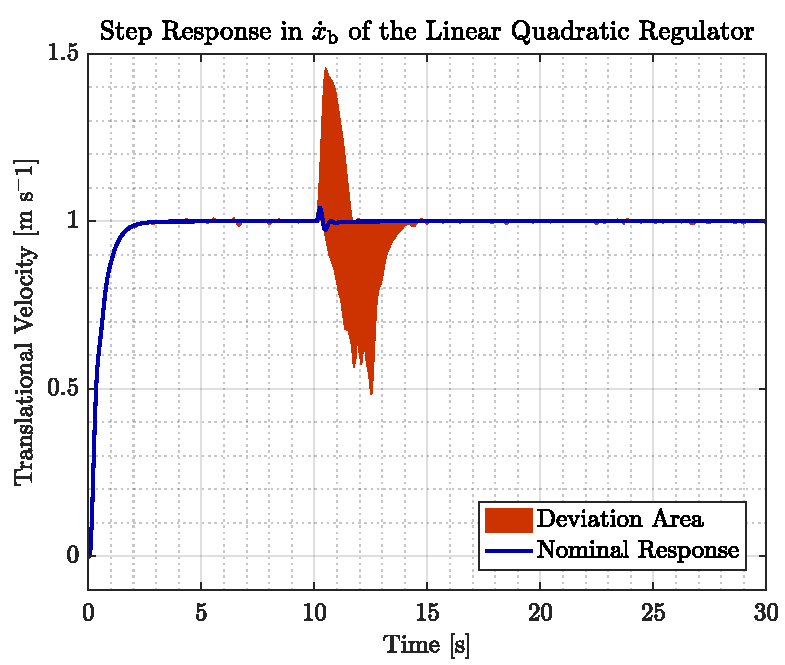
\includegraphics[width=.45\textwidth]{figures/xbdot_mc_lqr}         
    }                                                                    
    \hspace{5pt}                                                          
    \captionbox  
    {      
        Step response in $x_\mathrm{b}$ of the $\mathcal{H}_\infty$ controller, where the nominal response, the maximum variation region and the 1$\sigma$ region are shown.
        \label{fig:xbdot_mc_rob}
    }                                                                          
    {
        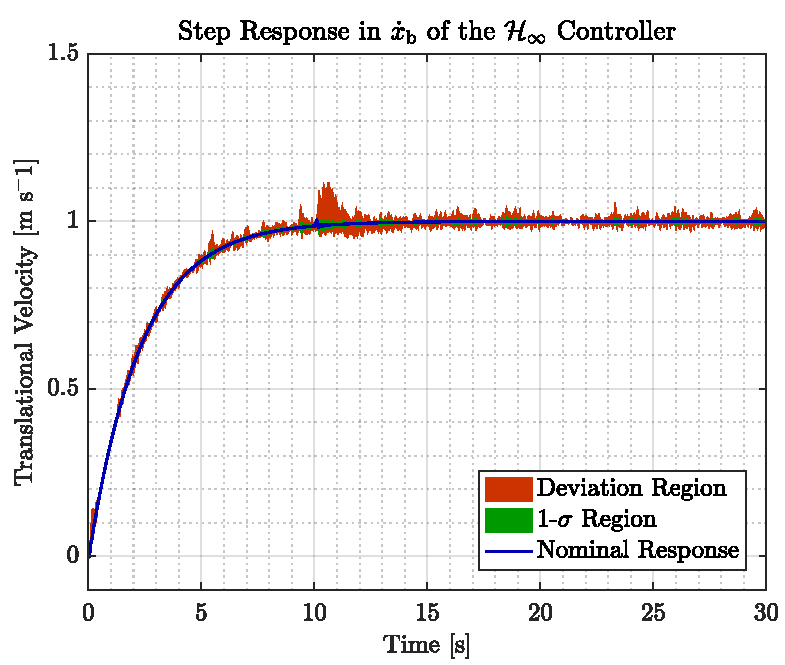
\includegraphics[width=.45\textwidth]{figures/xbdot_mc_rob}
    }
\end{figure}
As it can be seen, both controllers are able to track the given reference in $\dot{x}_\mathrm{b}$. The controller designed using LQR theory yields a fast controller, but the change in reference in the $\psi$ angle leads to a great perturbation in the vessel speed, reaching 50\% of deviation, while the 1$\sigma$ values go up to approximately 10\%. There is no steady state error once the perturbation has been compensated by the controller. 

The $\mathcal{H}_\infty$ controller on the other hand, is slower in terms of settling time. The perturbation introduced when changing $\psi_\mathrm{ref}$ has a 1$\sigma$ value that is almost zero and a maximum value around 15\%. This is acceptable as the forward velocity of the vessel does not require a fast response and it is not a critical parameter for the outer controller.

It can be seen that the LQR response has a settling time of 1 s, with an error band of 5\%, while the $\mathcal{H}_\infty$ controller takes around 5 s to settle. These responses can be approximated with first order systems with time constants of \num{0.33} s and \num{1.66} s, respectively, which give bandwidths \num{3} rad$\cdot$s$^{-1}$ and \num{0.6} rad$\cdot$s$^{-1}$.

In \autoref{fig:xbdot_mc_lqr_error} and \ref{fig:xbdot_mc_rob_error}, a closed look to the difference of the step responses with respect to the nominal behavior is shown.
\begin{figure}[H]
    \captionbox 
    {   
        Difference with the nominal behavior in $x_\mathrm{b}$ of the LQR, where the maximum variation region and the 1$\sigma$ region are shown.
        \label{fig:xbdot_mc_lqr_error}
    }                                                                 
    {                                                                  
        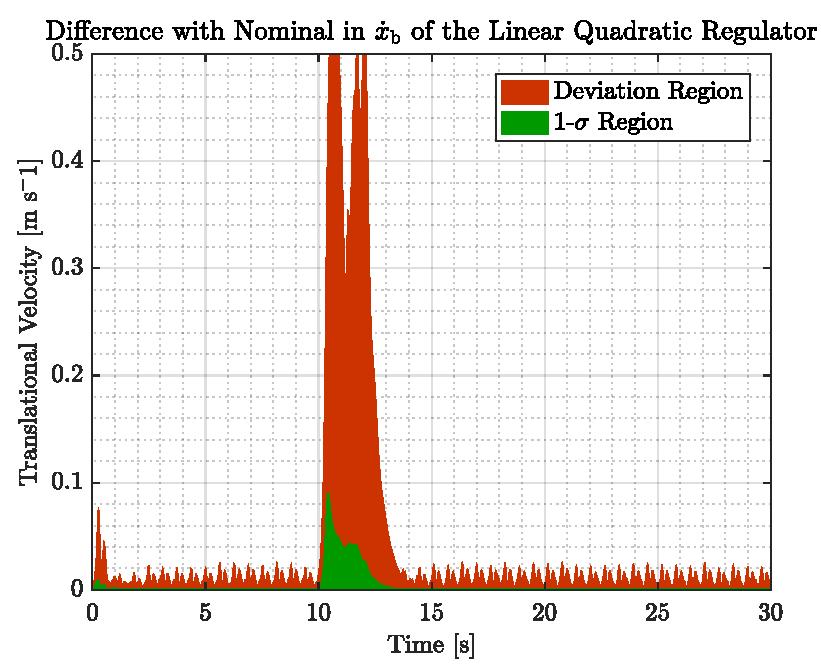
\includegraphics[width=.45\textwidth]{figures/xbdot_mc_lqr_error}         
    }                                                                    
    \hspace{5pt}                                                          
    \captionbox  
    {      
         Difference with the nominal behavior in $x_\mathrm{b}$ of the $\mathcal{H}_\infty$ controller, where the maximum variation region and the 1$\sigma$ region are shown.
        \label{fig:xbdot_mc_rob_error}
    }                                                                          
    {
        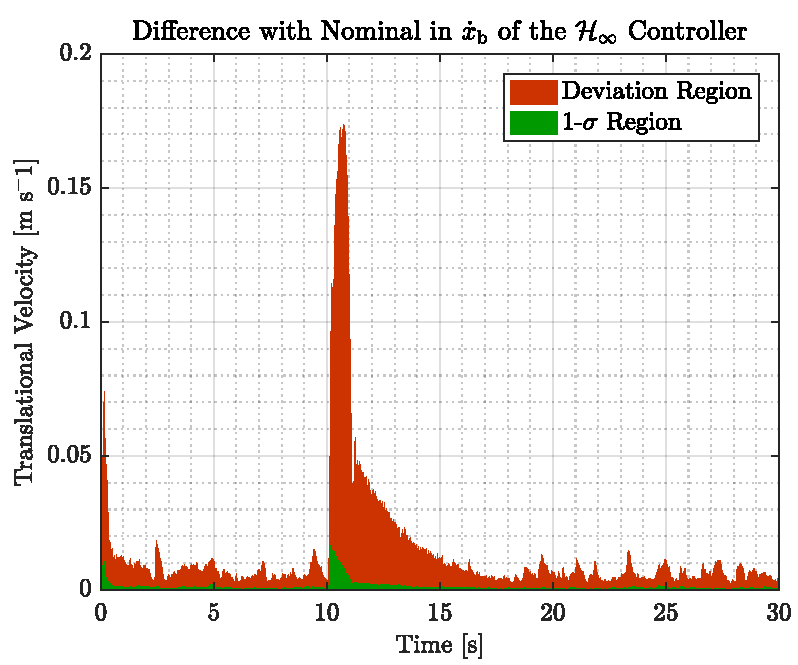
\includegraphics[width=.45\textwidth]{figures/xbdot_mc_rob_error}
    }
\end{figure}

It can be seen that the error keeps at a low value until the step for $\psi$ is applied and the highest disturbance occurs, being the $\mathcal{H}_\infty$ controller the one that is able to reject better the disturbance and the one with less variation from the nominal performance.

In \autoref{fig:yaw_mc_lqr} and \ref{fig:yaw_mc_rob}, the performance of the controllers is analyzed by looking at the step response when tracking a reference in $\psi$. These plots are part of the same simulations depicted in \autoref{fig:xbdot_mc_lqr} and \ref{fig:xbdot_mc_rob}, and therefore cope with the same disturbances and parameter variations. The step is applied after 10 seconds of simulation.
\begin{figure}[H]
    \captionbox 
    {   
        Step response in $\psi$ of the Linear Quadratic Regulator, where the nominal response, the maximum variation region and the 1$\sigma$ region are shown.
        \label{fig:yaw_mc_lqr}
    }                                                                 
    {                                                                  
        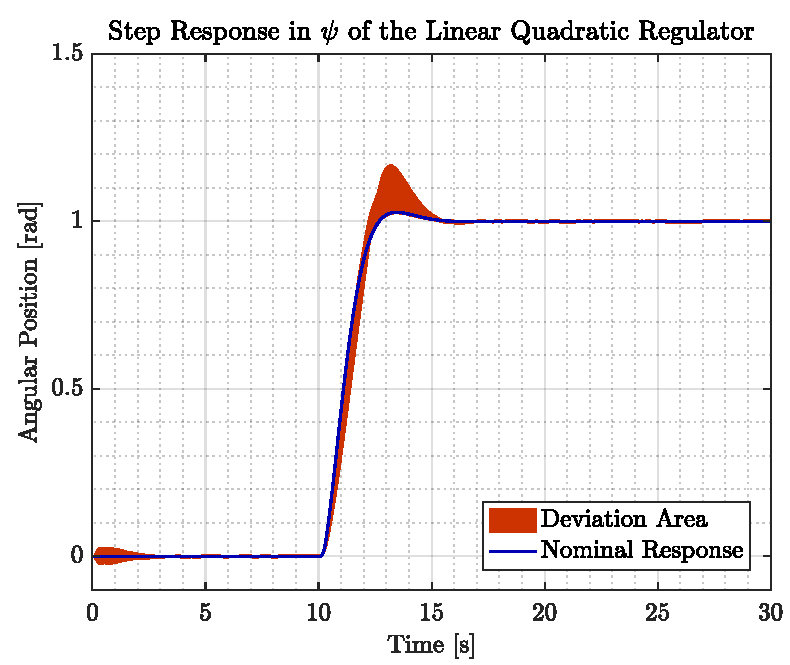
\includegraphics[width=.45\textwidth]{figures/yaw_mc_lqr}         
    }                                                                    
    \hspace{5pt}                                                          
    \captionbox  
    {   
        Step response in $\psi$ of the $\mathcal{H}_\infty$ controller, where the nominal response, the maximum variation region and the 1$\sigma$ region are shown.   
        \label{fig:yaw_mc_rob}
    }                                                                          
    {
        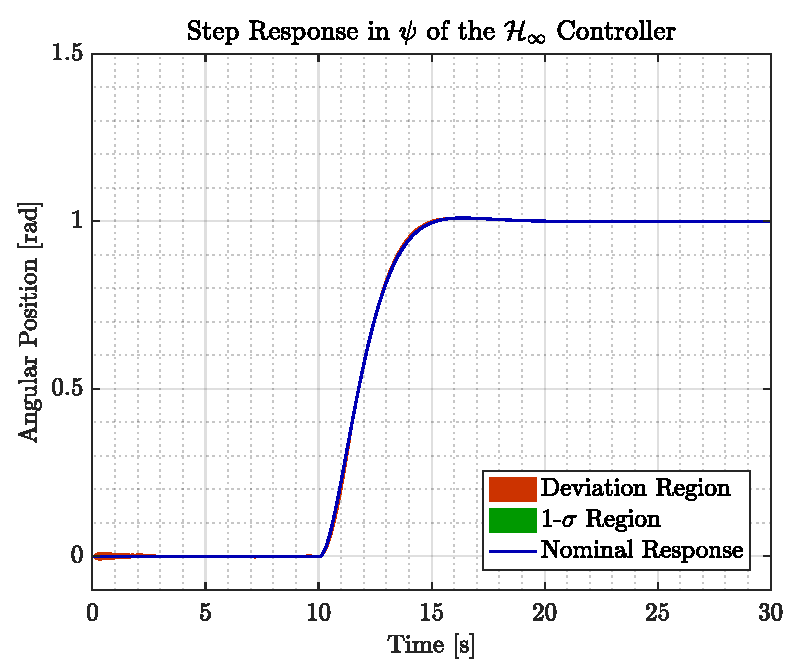
\includegraphics[width=.45\textwidth]{figures/yaw_mc_rob}
    }
\end{figure}

The behavior seen in these figures resembles that for \autoref{fig:xbdot_mc_lqr} and \ref{fig:xbdot_mc_rob}. The $\mathcal{H}_\infty$ controller shows less overshoot and variability in the different simulations but it is also slightly slower than the LQR controller. In both cases, the 1$\sigma$ value is very closed to zero, but the response of the LQR shows a maximum variation of 20\%.

Additionally, it can be seen that the LQR response has a settling time of 2 s, while the $\mathcal{H}_\infty$ controller takes around \num{3.5} s to settle. These responses can be approximated with first order systems with time constants of \num{0.66} s and \num{1.16} s, respectively, which give bandwidths \num{1.5} rad$\cdot$s$^{-1}$ and \num{0.86} rad$\cdot$s$^{-1}$.

As in the case of $\dot{x}_\mathrm{b}$, a close look at the difference with respect to the nominal response can be seen in \autoref{fig:yaw_mc_lqr_error} and \ref{fig:yaw_mc_rob_error}.
\begin{figure}[H]
    \captionbox 
    {   
        Difference with the nominal behavior in $\psi$ of the LQR, where the maximum variation region and the 1$\sigma$ region are shown.
        \label{fig:yaw_mc_lqr_error}
    }                                                                 
    {                                                                  
        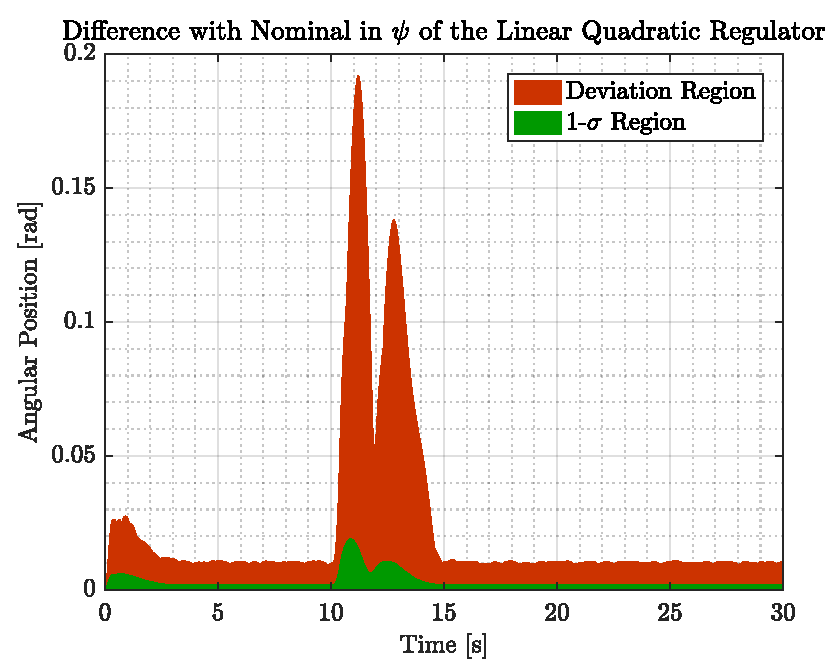
\includegraphics[width=.45\textwidth]{figures/yaw_mc_lqr_error}         
    }                                                                    
    \hspace{5pt}                                                          
    \captionbox  
    {   
        Difference with the nominal behavior in $\psi$ of the $\mathcal{H}_\infty$ Controller, where the maximum variation region and the 1$\sigma$ region are shown.   
        \label{fig:yaw_mc_rob_error}
    }                                                                          
    {
        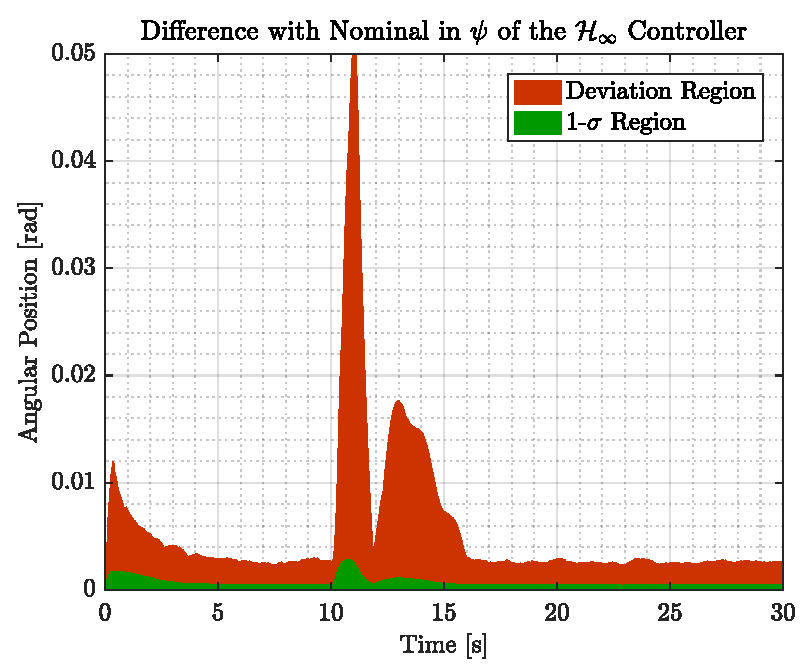
\includegraphics[width=.45\textwidth]{figures/yaw_mc_rob_error}
    }
\end{figure}

In this case, it is also the $\mathcal{H}_\infty$ Controller the one that is able to handle better the disturbances and with less variations with respect to the nominal behavior.

These controller designs are also compared by their usage of inputs. The mean force applied at each time by the thrusters when simulating the LQR controller is \num{17.5793} N, while that of the $\mathcal{H}_\infty$ controller is \num{17.9281} N. This results as expected since the Linear Quadratic Regulator is designed to optimize the use of inputs to the system.

Finally, to combine performance and usage of inputs, the cost used in the LQR design is calculated using \autoref{eq:cost}. The mean cost among the simulations is \num{7.1441}$\cdot 10^5$ and \num{3.4227}$\cdot 10^6$ for the LQR and $\mathcal{H}_\infty$ controller designs, respectively. As expected, the cost is lower for the LQR design as minimizing it is the basis of the LQR approach.



